\part{Progettazione di un'interfaccia grafica per la compressione di immagini}

L'interfaccia grafica è realizzata con l'ambiente di sviluppo Qt\cite{qt}, il quale permette di creare delle GUI scrivendo il codice in linguaggio C++. La compressione applicata è stata limitata solamente alla visualizzazione, ovvero l'immagine perde l'informazione legata alle alte frequenze, però le strutture dati che contengono tale immagine rimangono costanti. Introducendo la possibilità, ad un successivo salvataggio dell'immagine, di memorizzare solamente i coefficienti diversi da 0, richiamando un concetto di simil sparsità però applicato alle frequenze non tagliate dalla compressione.

Il programma fornisce una schermata nella quale è possibile selezionare l'immagine da comprimere e i valori di compressione da applicare, ossia dimensione dei blocchi e la soglia di taglio delle frequenze. Nella parte sinistra della GUI viene mostrata l'immagine originale, mentre in quella di destra la sua versione compressa. In figura\ref{fig:deer} è riportato un esempio sull'immagine \textit{deer}, sulla quale sono stati applicati blocchi di elevate dimensioni (70x70) ed una elevata compressione (circa del 92\%), in questo modo è facilmente osservabile l'effetto della compressione sui blocchi e sull'immagine.

\begin{figure}[h]
	\centering
	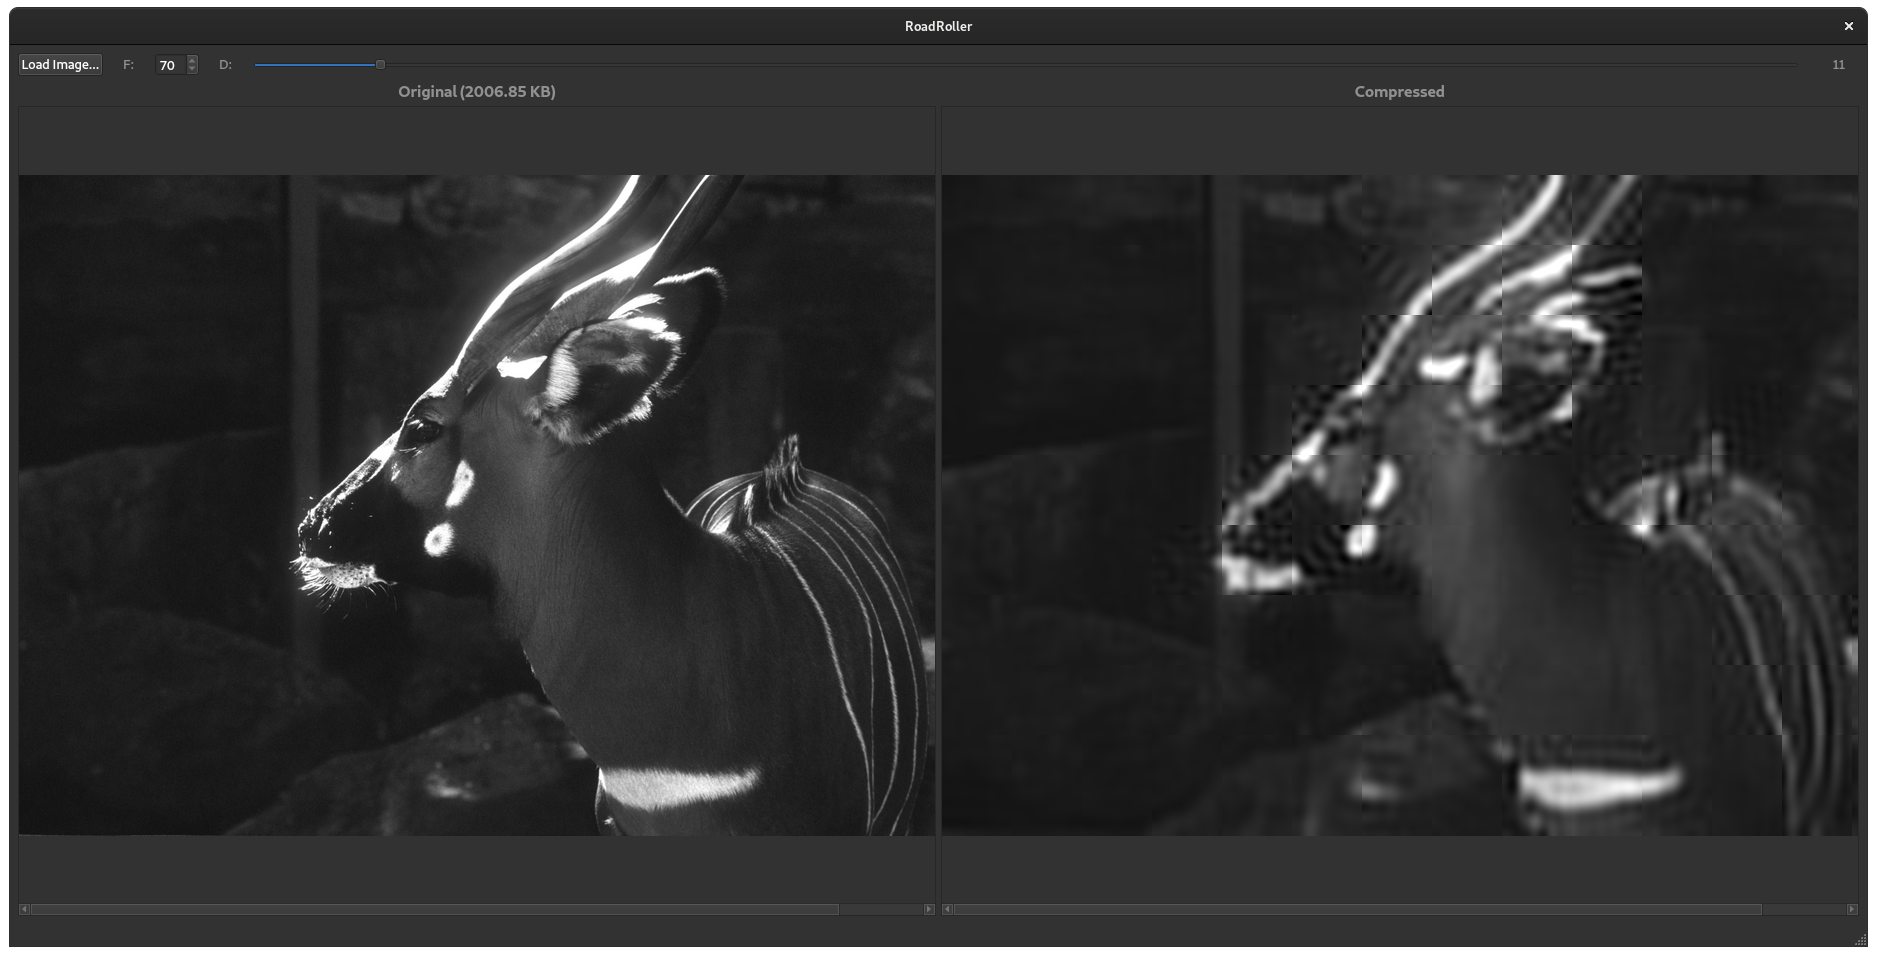
\includegraphics[width=1\linewidth]{figures/qt_deer}
	\caption{Programma di compressione basato su Qt}
	\label{fig:deer}
\end{figure}

\section{Features}

Alla versione base del progetto, descritto precedentemente, sono state aggiunte un insieme di funzionalità:

\begin{itemize}
	\item \textbf{Multithreading}: L'aggiunta dei thread permette una rapida compressione dell'immagine. Infatti essendo che i blocchi lavorano su aree della figura indipendenti gli uni dagli altri, è possibile eseguire le compressioni in parallelo, così come la scrittura dei pixel nell'oggetto immagine finale.
	
	Abbiamo fatto in modo che i blocchi vengano suddivisi in una griglia la cui quantità di celle di celle corrisponde al numero di core del sistema. In questo modo, il carico di lavoro può essere distribuito in modo equo tra i processori e minimizzare il tempo di esecuzione della compressione.
	\item \textbf{Navigazione dell'immagine}: All'interno dell'interfaccia grafica sono presenti degli slider e dei tasti per zoomare nelle immagine, tali tasti sono sincronizzati in modo tale da poter visionare contemporaneamente le stesse zone delle 2 immagini. In questo modo si possono osservare più comodamente i vari effetti che la compressione comporta sulle immagini.
	\item \textbf{Aggiornamento in tempo reale}: Grazie ai thread, che velocizzano notevolmente il lavoro, modificando la dimensioni dei blocchi e/o la dimensione del taglio delle frequenze, é possibile visionare nella parte di destra gli aggiornamenti sulla compressione, in tempo reale. Il delay che intercorre tra la modifica del parametro e il suo aggiornamento é solitamente molto basso, anche se ovviamente varia in relazione alla dimensione dell'immagine passata in input.
	\item  \textbf{Gestione dei bordi}:  A fini sperimentali, abbiamo provato ad implementare il processo di compressione in modo che venga effettuata la dct anche su blocchi più piccoli sui bordi dell'immagine, in modo da ricoprirne l'intera superficie.
\end{itemize}

\section{Gestione dei pixel in eccesso}

All'interno di questo progetto, abbiamo deciso in modo "sperimentale" di gestire in maniera leggermente diversa da jpeg i pixel sui margini.

Nello specifico, il nostro programma di compressione considera i pixel in eccesso derivati dalla suddivisione in blocchi e li utilizza per creare dei blocchi più piccoli, al fine di riempire l'intera immagine. Dopo questa operazione, ne esegue la DCT2 allo stesso modo degli altri blocchi. Prima di eseguire il taglio, però, il valore del taglio viene adattato in modo da essere proporzionato alla minore quantità di frequenze e da rendere, quindi, la compressione dell'immagine più uniforme:

$$d' = \floor*{d  \sqrt{ \frac{W \cdot H}{F^{2}}}}$$

dove W e H rappresentano rispettivamente la larghezza e l'altezza del blocco preso in considerazione.
Inoltre, nel caso in cui $d'=0$, ma $d>0$, si mantiene il valore 1 al fine di evitare buchi indesiderati.

Abbiamo preso questa decisione perché, a differenza di jpeg, non siamo stati vincolati dalla matrice di quantizzazione e abbiamo potuto, quindi, sperimentare una gestione leggermente diversa del margine dell'immagine.


\begin{figure}
	\begin{minipage}{0.5\textwidth}
		\begin{center}
		
			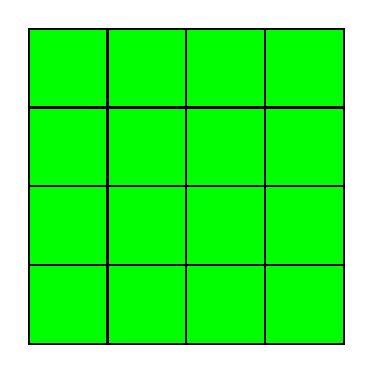
\begin{tikzpicture}
				[%%%%%%%%%%%%%%%%%%%%%%%%%%%%%%
				box/.style={rectangle,draw=black,thick, minimum size=1cm},
				]%%%%%%%%%%%%%%%%%%%%%%%%%%%%%%
				
				\foreach \x in {0,1,...,3}{
					\foreach \y in {0,1,...,3}
					\node[box, fill=red] at (\x,\y){};
				}
			
			
				\foreach \x in {0,...,3}{
					\foreach \y in {0,...,3} {
						\ifnumcomp{\x + (3 - \y)}{<}{5}{
							\node[box, fill=green] at (\x,\y){};
						}{};
					}
				}
				
				
			\end{tikzpicture}
		\end{center}
		\begin{center}
			(a)
		\end{center}
	\end{minipage}\hfill
	\begin{minipage}{0.5\textwidth}
		\begin{center}
			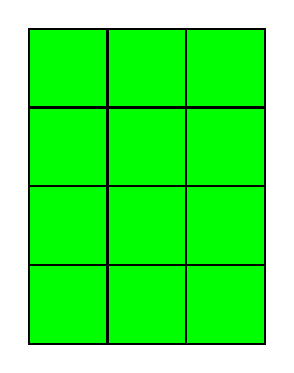
\begin{tikzpicture}
				[%%%%%%%%%%%%%%%%%%%%%%%%%%%%%%
				box/.style={rectangle,draw=black,thick, minimum size=1cm},
				]%%%%%%%%%%%%%%%%%%%%%%%%%%%%%%
				
				\foreach \x in {0,1,...,2}{
					\foreach \y in {0,1,...,3}
					\node[box, fill=red] at (\x,\y){};
				}
				
				
				\foreach \x in {0,...,2}{
					\foreach \y in {0,...,3} {
						\ifnumcomp{\x + (3 - \y)}{<}{5}{
							\node[box, fill=green] at (\x,\y){};
						}{};
					}
				}
				
				
			\end{tikzpicture}
		\end{center}
	\begin{center}
		(b)
	\end{center}
\end{minipage}
\caption{Taglio delle frequenze sulle diverse dimensioni dei blocchi}\label{fig:taglio}
\end{figure}

\section{Visualizzazione dei risultati}

Per mostrare meglio la compressione potremmo momentaneamente ignorare la conversione dei valori tramite la IDCT2. In figura\ref{fig:compression_values} viene mostrato il risultato ottenuto, dove è possibile osservare i coefficienti generati dalla DCT, i quali vengono successivamente tagliati per il valore di input scelto. In questo modo, ogni blocco conterrà dati diversi da 0 solo nella parte superiore del taglio, evidenziata anche graficamente dalla distribuzione del colore bianco nei singoli blocchi. Infatti tale tonalità rappresenta un valore elevato del coefficiente presente nella matrice, mentre le zone nere, rappresentano i valori che sono stati impostati a 0 dal taglio.

\begin{figure}[h]
	\centering
	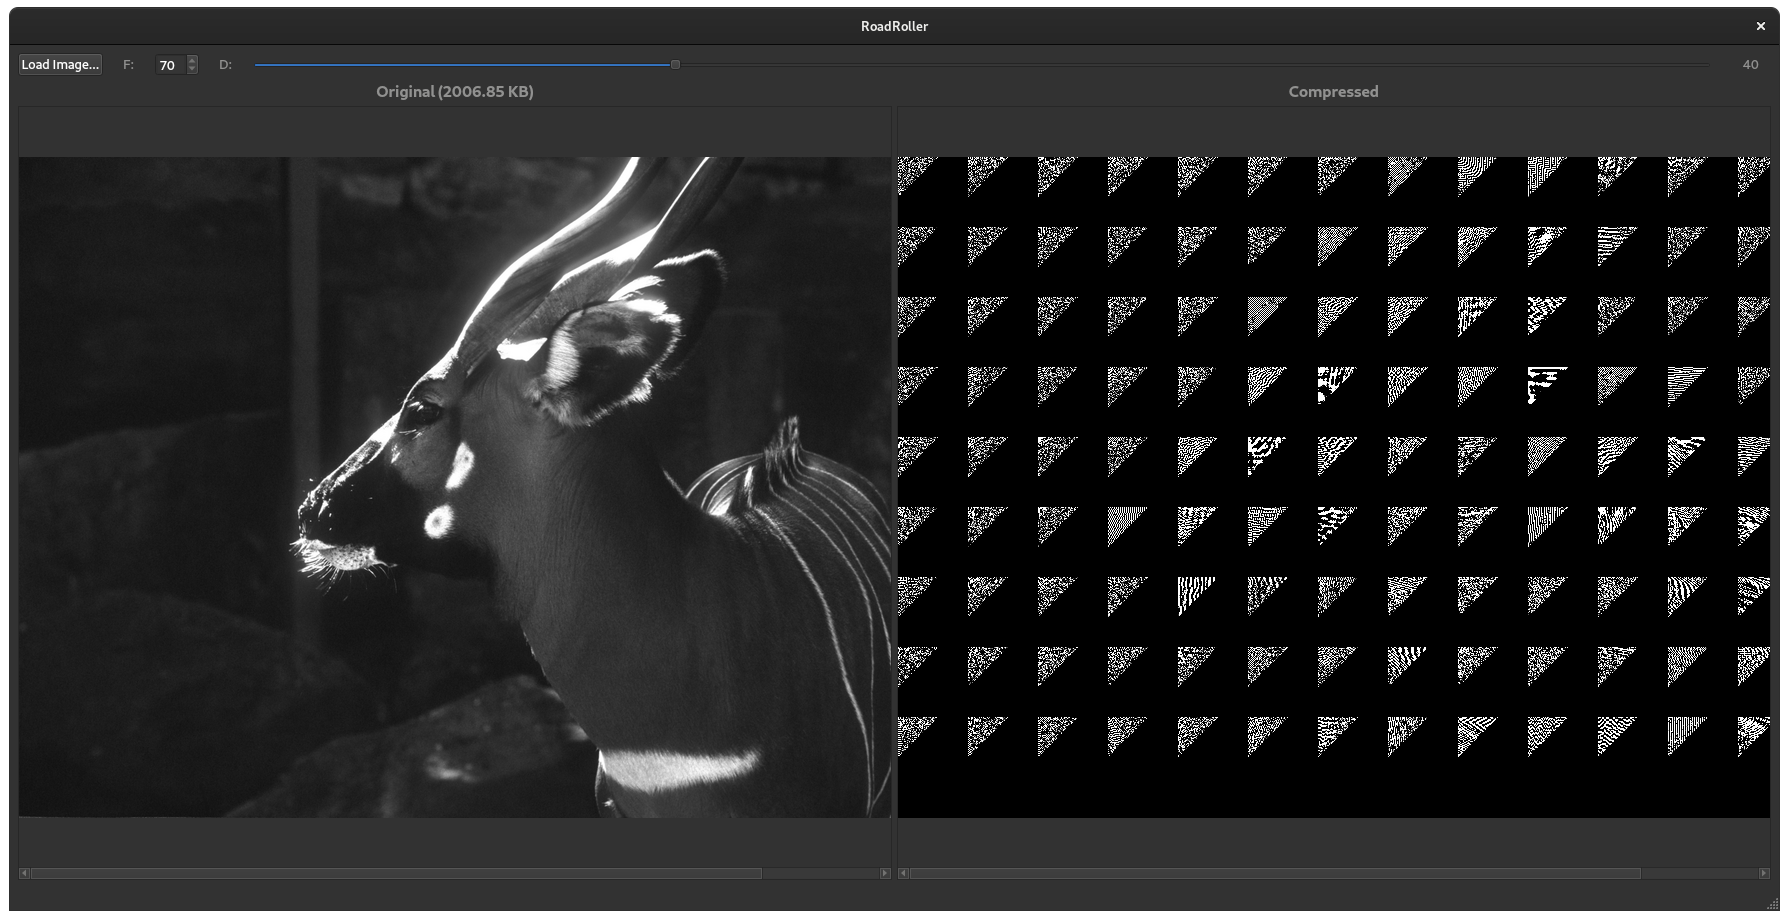
\includegraphics[width=1\linewidth]{figures/qt_dct_values}
	\caption{Valori della DCT generati dalla compressione (a meno dello scaling)}
	\label{fig:compression_values}
\end{figure}

\subsection{Fenomeno di Gibbs}

Scegliendo un'elevata dimensione dei blocchi si ottiene comunque il fenomeno di Gibbs, visibile chiaramente in Figura \ref{fig:gibbs}. Dove l'elevato contrasto tra il muso del cervo e il relativo sfondo, generano un repentino cambio di colore, il quale comporta l'apparizione degli artefatti sotto forma di onde nell'immagine finale.

Per rappresentare meglio il fenomeno, nel grafico di Figura \ref{fig:dct_values_on_gibbs} sono stati rappresentati i coefficienti della DCT relativi al blocco precedentemente illustrato, che presenta tale fenomeno. Per una migliore visualizzazione, la scala è stata ristretta, in questo modo non è possibile osservare la totalità del peso delle basse frequenze, ma in compenso si osserva meglio la distribuzione dei coefficienti su tutte le restanti frequenze.

Nell'istogramma le basse frequenze hanno valori nell'ordine di \path{1e+6}, mentre allontanandosi troviamo coefficienti che sono in proporzione molto più piccoli (nell'ordine delle migliaia), visibili in Figura \ref{fig:last_dct_values_gibbs}. Tali valori però sono fondamentali nella corretta rappresentazione dell'immagine, infatti essi riescono a modellare il repentino cambio di colore presente nel blocco analizzato. Quindi nel momento in cui essi vengono tagliati dalla compressione, si ottiene il fenomeno illustrato precedentemente in Figura \ref{fig:gibbs}

\begin{figure}[h]
	\centering
	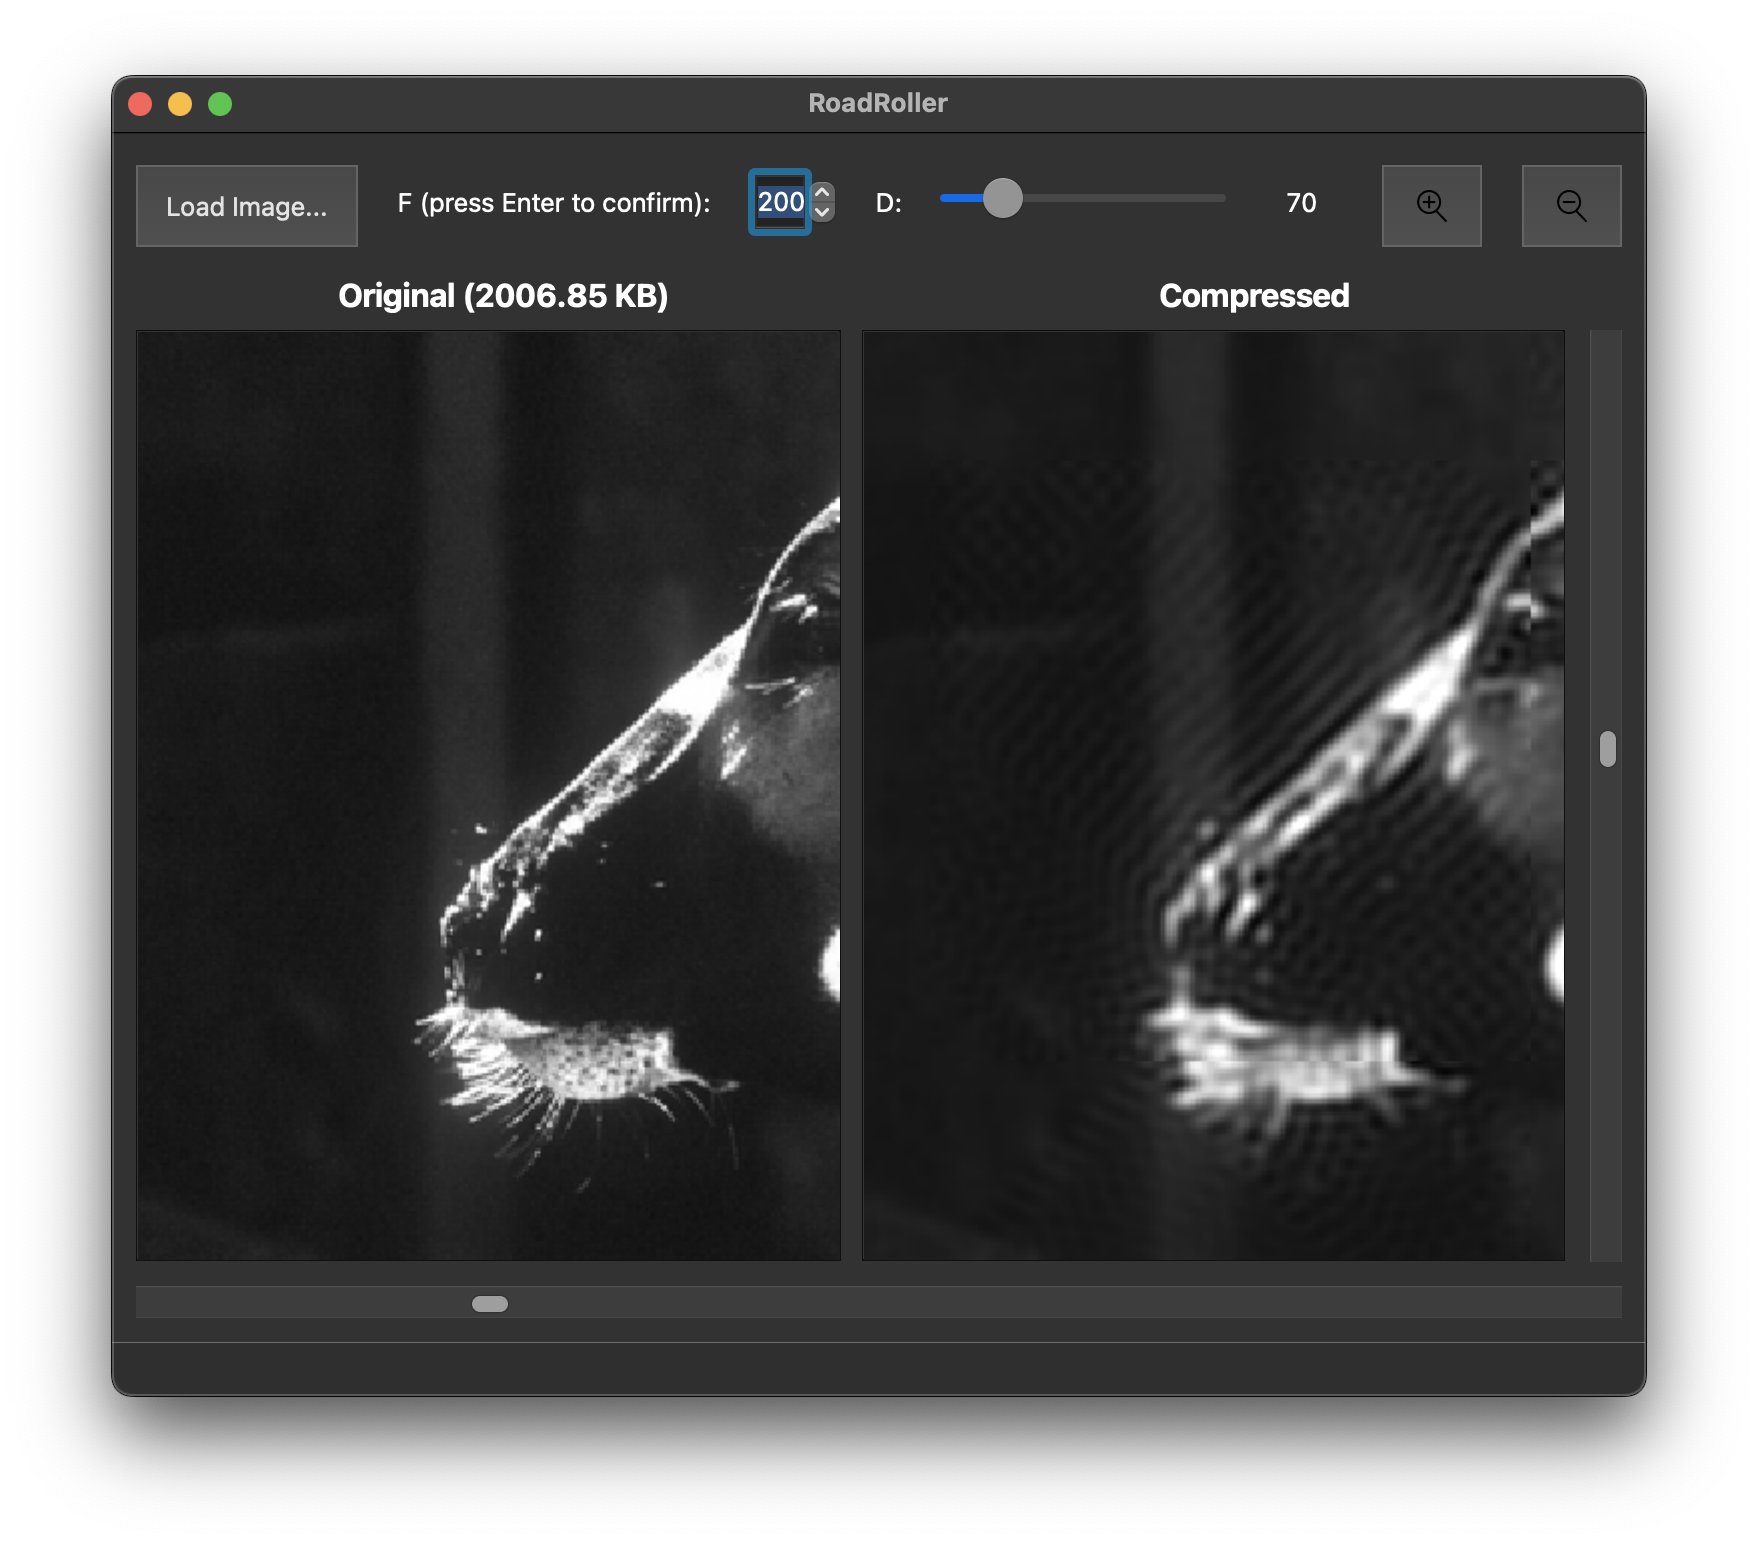
\includegraphics[width=1\linewidth]{figures/gibbs_phenomenon}
	\caption{Fenomeno di Gibbs su un blocco}
	\label{fig:gibbs}
\end{figure}


\begin{figure}
	\centering
	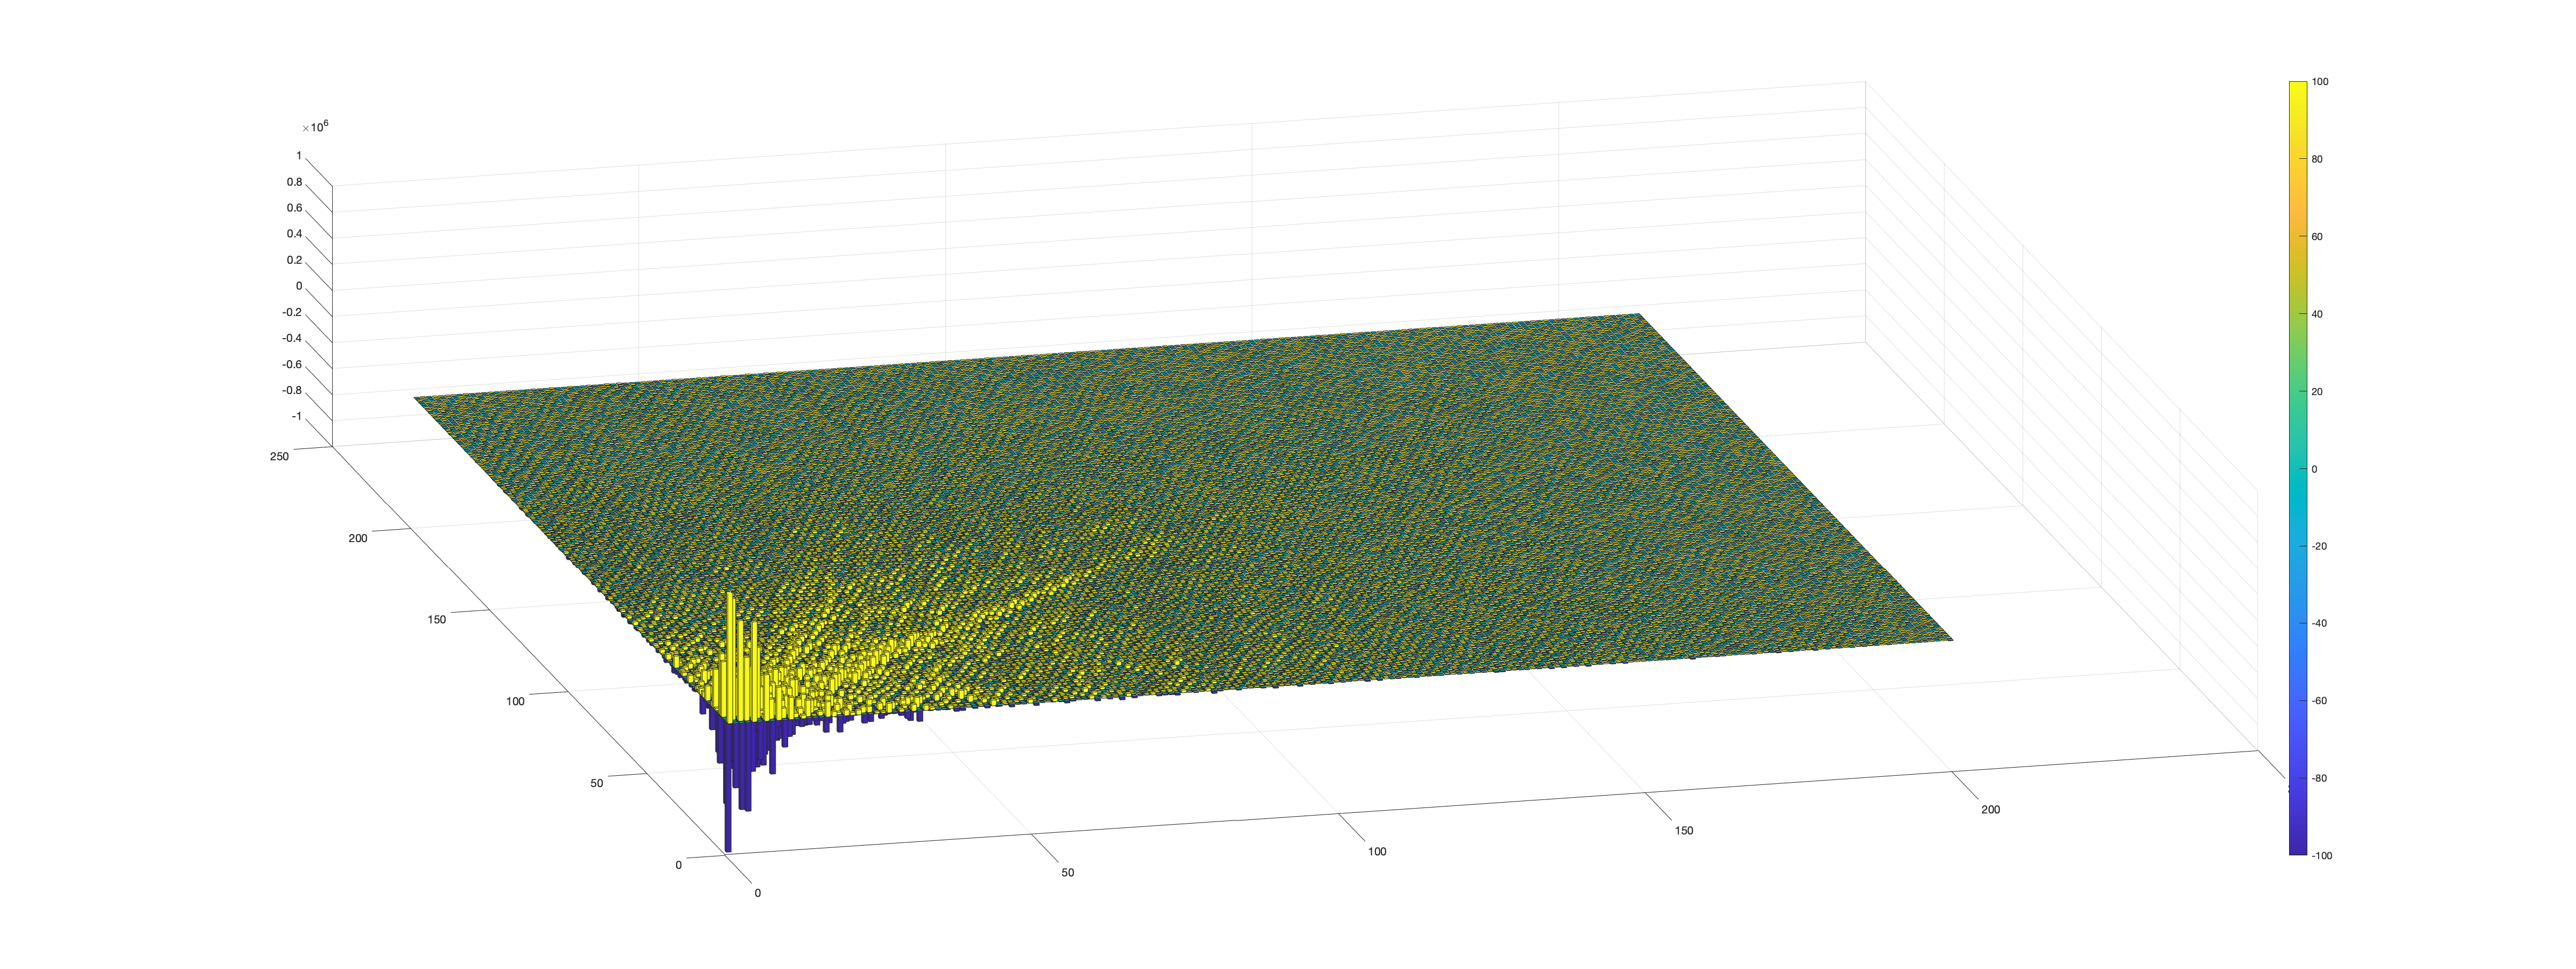
\includegraphics[width=1\linewidth]{figures/dct_values_3d.eps}
	\caption{Coefficienti DCT nel blocco mostrato in Figura \ref{fig:gibbs}}
	\label{fig:dct_values_on_gibbs}
\end{figure}

\begin{figure}
	\centering
	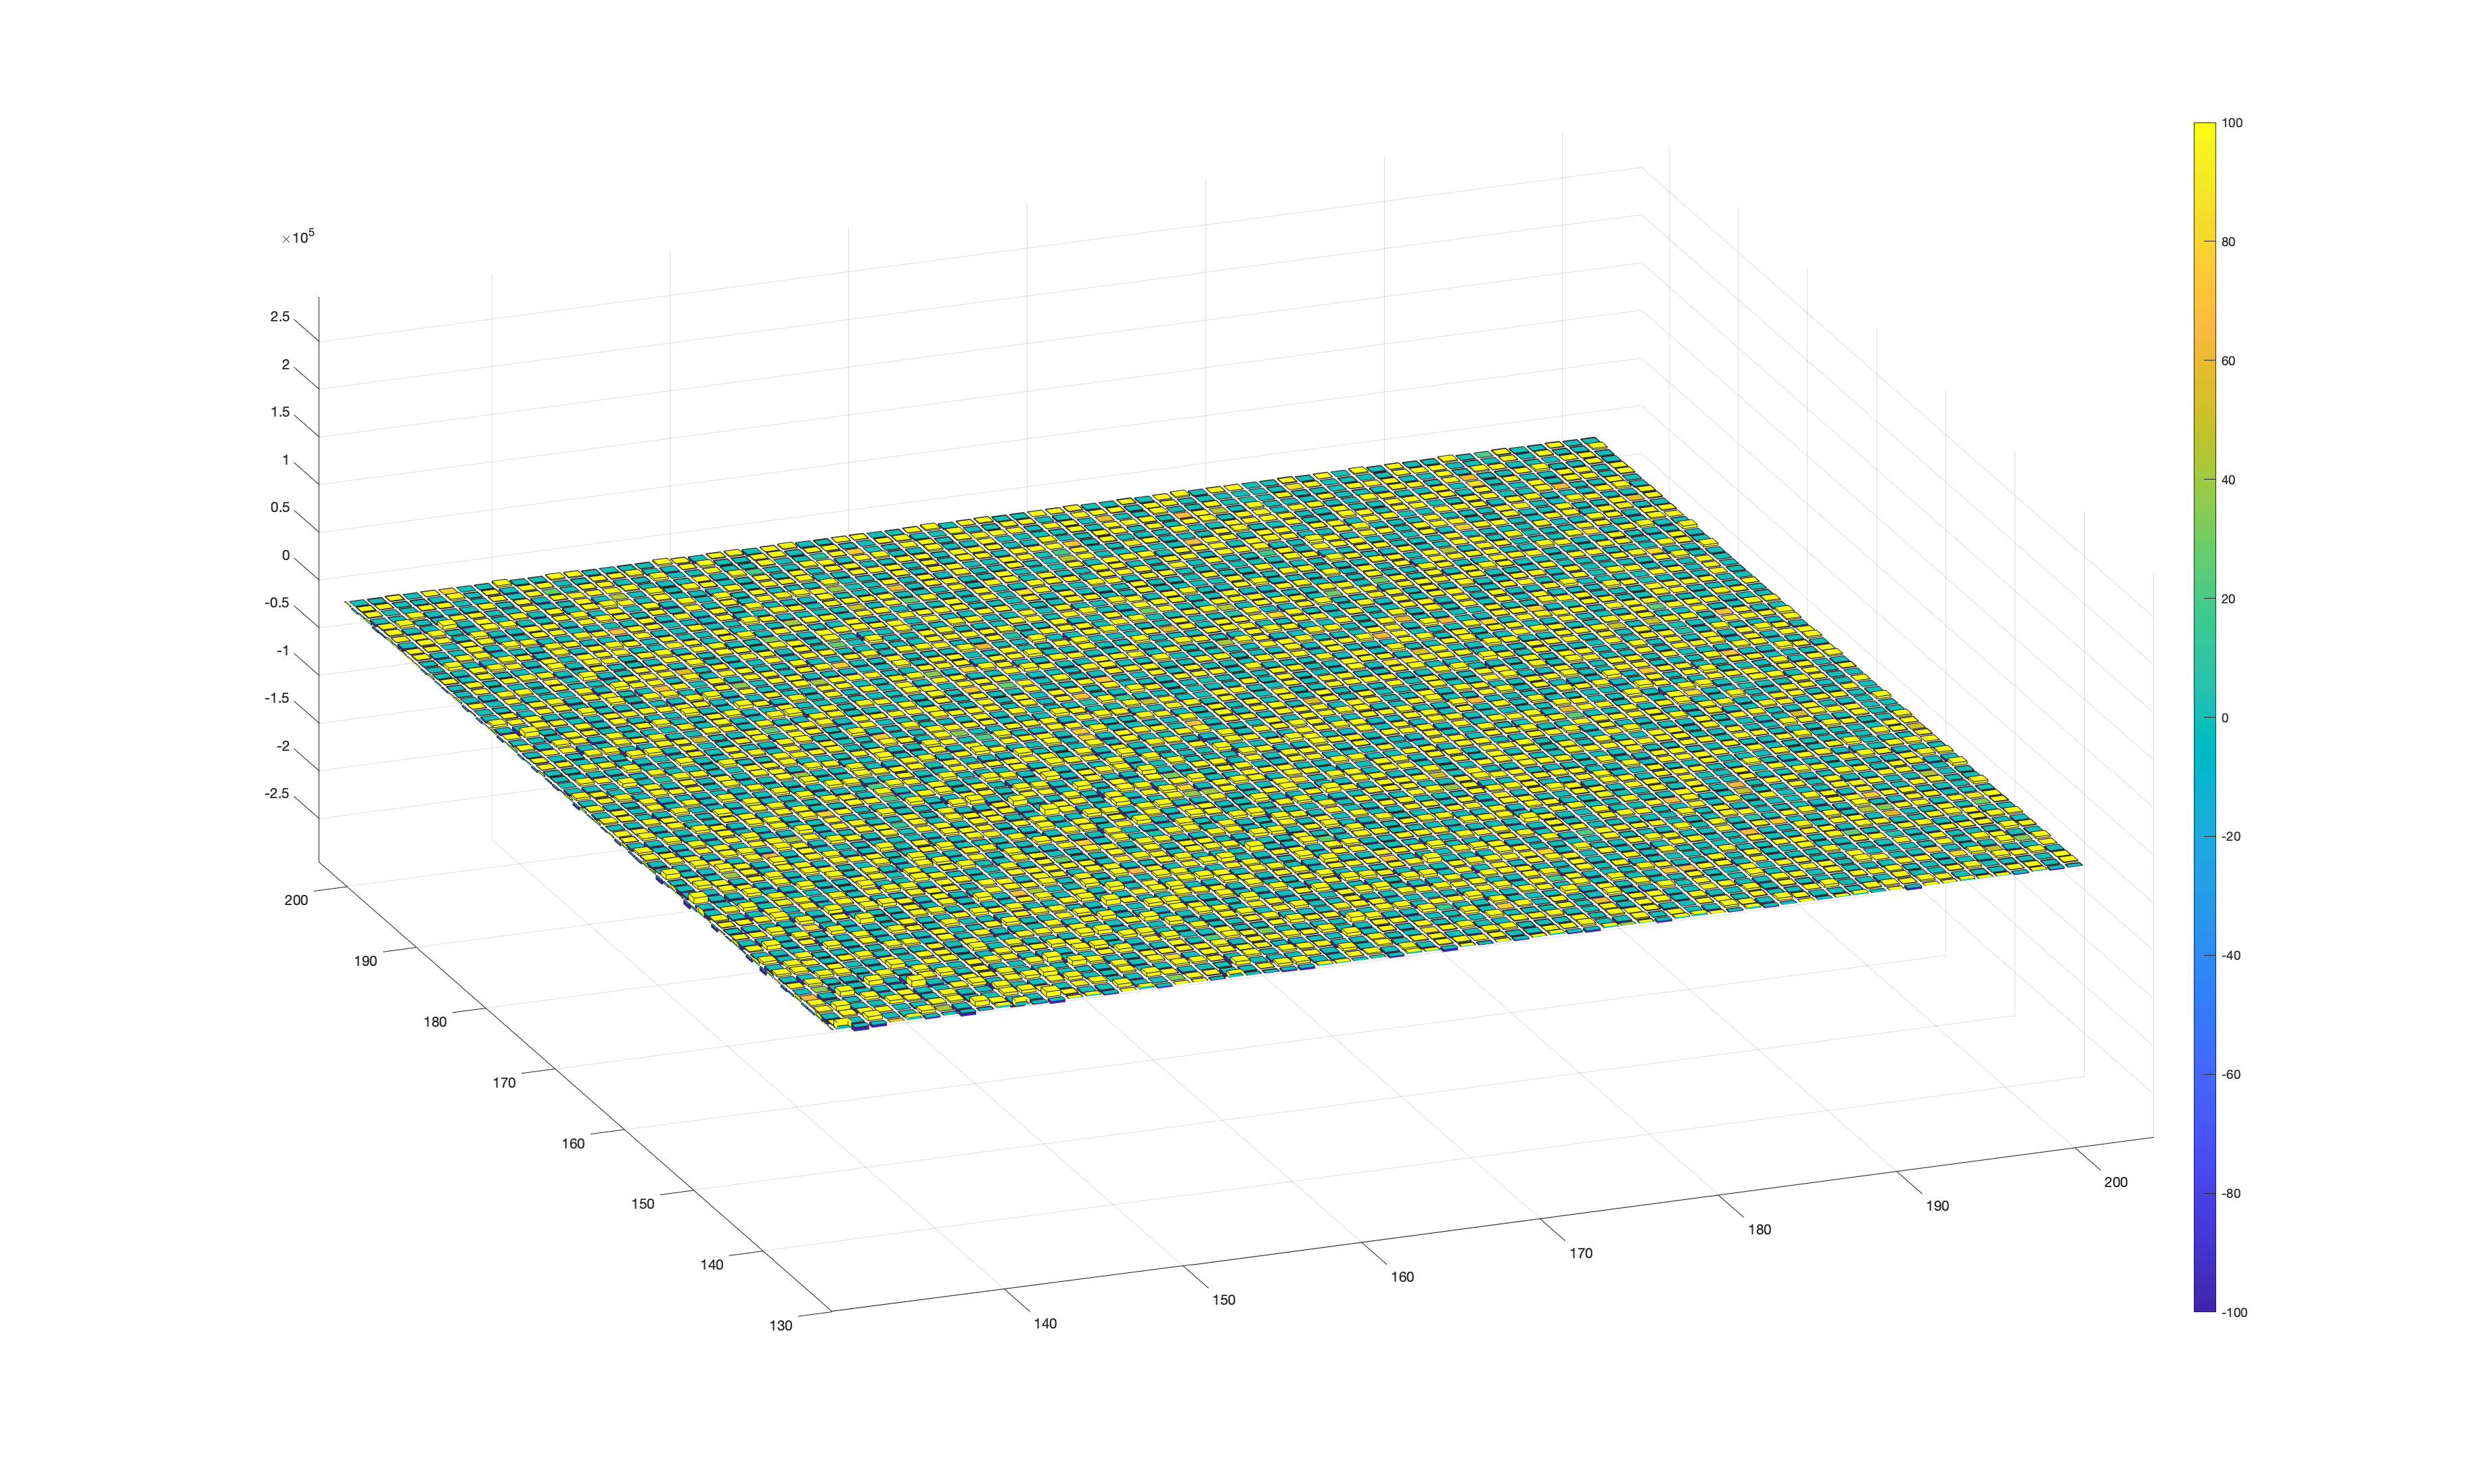
\includegraphics[width=1\linewidth]{figures/last_dct_values.eps}

	\caption{Ultimi 50 x 50 coefficienti della DCT relativi alla Figura \ref{fig:dct_values_on_gibbs}}
	\label{fig:last_dct_values_gibbs}
\end{figure}